%% LaTeX Beamer presentation template (requires beamer package)
%% see http://bitbucket.org/rivanvx/beamer/wiki/Home
%% idea contributed by H. Turgut Uyar
%% template based on a template by Till Tantau
%% this template is still evolving - it might differ in future releases!

\documentclass{beamer}

\mode<presentation>
{
\usetheme{Warsaw}

\setbeamercovered{transparent}
}

\usepackage[english]{babel}
\usepackage[latin1]{inputenc}

% font definitions, try \usepackage{ae} instead of the following
% three lines if you don't like this look
\usepackage{mathptmx}
\usepackage[scaled=.90]{helvet}
\usepackage{courier}


\usepackage[T1]{fontenc}


\title{Optisches Pumpen}

\subtitle{Fortgeschrittenen-Praktikum II}

% - Use the \inst{?} command only if the authors have different
%   affiliation.
%\author{F.~Author\inst{1} \and S.~Another\inst{2}}
\author{\inst{1}}

% - Use the \inst command only if there are several affiliations.
% - Keep it simple, no one is interested in your street address.
\institute[Universities of]
{
\inst{1}%
Department of Computer Science\\
Univ of S
\and
\inst{2}%
Department of Theoretical Philosophy\\
Univ of E}

\date{18.05.2015}


% This is only inserted into the PDF information catalog. Can be left
% out.
\subject{Talks}

% Delete this, if you do not want the table of contents to pop up at
% the beginning of each subsection:
\AtBeginSubsection[]
{
\begin{frame}<beamer>
\frametitle{Outline}
\tableofcontents[currentsection,currentsubsection]
\end{frame}
}

% If you wish to uncover everything in a step-wise fashion, uncomment
% the following command:

%\beamerdefaultoverlayspecification{<+->}

\begin{document}

\begin{frame}
\titlepage
\end{frame}

\begin{frame}
\frametitle{Outline}
\tableofcontents
% You might wish to add the option [pausesections]
\end{frame}

%%% BEN 5' %%%

\section{Allgemeine Grundlagen}

\subsection{Die Hyperfeinstruktur}

\begin{frame}
\frametitle{Hyperfeinstruktur-Aufspaltung}
\begin{itemize}
    \item<1-> Kopplung von Kernspin $\vec{I}$ und elektronischem Gesamtdrehimpuls $\vec{J}$
    \begin{equation*}
        \vec{F} = \vec{I} + \vec{J} \qquad \qquad \abs{I - J} \leq F \leq \abs{I + J}
    \end{equation*}
    \item<2-> Energieaufspaltung
    \begin{equation*}
        \Delta E_\text{HFS} = - \vec{\mu}_I \cdot \vec{B}_J
    \end{equation*}
    \item<3-> Für benachbarte Energieniveaus
    \begin{equation*}
        \Delta E_{\Delta F = 1} (F) = A(F+1)
    \end{equation*}
    Intervallkonstante $A$
\end{itemize}
\end{frame}


\begin{frame}
\frametitle{Hyperfeinstruktur-Aufspaltung von Rubidium}
\setbeamerfont{myfont}{size*=80}
\usebeamerfont{myfont}

\begin{figure}
    \centering
    \def\svgwidth{\textwidth}
    \input{../img/termschemahyperfein.pdf_tex}
    \caption{Hyperfeinstrukturaufspaltung der D$_1$-Linie von \rb{85} und \rb{87}.}
\end{figure}
\end{frame}


\begin{frame}
\frametitle{Hyperfeinstruktur-Aufspaltung - Übergänge}
\setbeamerfont{myfont}{size*=80}
\usebeamerfont{myfont}

\begin{figure}
    \centering
    \def\svgwidth{\textwidth}
    \input{../img/termschemahyperfein_linien.pdf_tex}
    \caption{Hyperfeinstrukturaufspaltung der D$_1$-Linie von 
    \rb{85} und \rb{87}.}
\end{figure}
\end{frame}

 


\begin{frame}
\frametitle{Hyperfeinstruktur-Aufspaltung - Spektrallinien}
\setbeamerfont{myfont}{size*=80}
\usebeamerfont{myfont}

\begin{figure}
    \centering
    \def\svgwidth{\textwidth}
    \input{../img/HFSspect_theo.pdf_tex}
    \caption{Spektrallinien der Hyperfeinstruktur des ${}^2\text{S}_{1/2}$\,-\,${}^2\text{P}_{1/2}$\,-\,Übergangs
    von \rb{85} und \rb{87}.}
\end{figure}

\end{frame}

\begin{frame}
\frametitle{Zeeman-Aufspaltung der Hyperfeinstruktur}
\begin{itemize}
    \item<1-> ohne Magnetfeld: Niveau ist $(2F+1)$-fach entartet
    \begin{equation*}
        F_z = m_F \hbar \qquad \qquad -F \leq m_F \leq F
    \end{equation*}
    \item<2-> mit äußerem Magnetfeld $\vec{B}_0$: Zeeman-Aufspaltung
    \item<3-> Für benachbarte Energieniveaus
    \begin{equation*}
        \Delta E_\text{HFS}^\text{Zeeman}(\Delta m_F = 1) = \frac{g_J \mu_B}{2 \left( I + \frac{1}{2} \right) } B_0
    \end{equation*}
    Bohrsches Magneton $\mu_B$, Landé-Faktor $g_J$
\end{itemize}
\end{frame}

\begin{frame}
\frametitle{Zeeman-Aufspaltung der Hyperfeinstruktur}

\setbeamerfont{myfont}{size*=80}
\usebeamerfont{myfont}

\begin{figure}
    \centering
    \def\svgwidth{\textwidth}
    \input{../img/termschema.pdf_tex}
    \caption{Zeeman-Aufspaltung der Hyperfeinstruktur von \rb{85} und \rb{87}.}
\end{figure}

\end{frame}




%%% MORITZ 2.5' %%%

\subsection{Die Laserdiode}

\begin{frame}
\frametitle{Laserdiode - Aufbau zur Charakterisierung}
\setbeamerfont{myfont}{size*=80}
\usebeamerfont{myfont}
\begin{figure}
    \centering
    \def\svgwidth{\textwidth}
    \input{../img/aufbauLaser.pdf_tex}
    \caption{Aufbau zur Messung der $P$-$I$-Kennlinie der Laserdiode.}
\end{figure}
\usebeamerfont{standard}
\begin{itemize}
  \item \textbf{Peltierelement:} Temperaturstabilisierung der Laserdiode
  \item \textbf{Laserdiode:} Erzeugung von linear polarisiertem kohärenten Licht mit $\lambda=500$\,nm
  \item \textbf{Neutraldichtefilter:} Abschwächung der Laserintensität
  \item \textbf{Photodiode:} Messung der Laserintensität
\end{itemize}
\end{frame}

\begin{frame}
\frametitle{Laserdiode - $P$-$I$-Kennlinie}

\begin{figure}[H]
    \begin{center}
        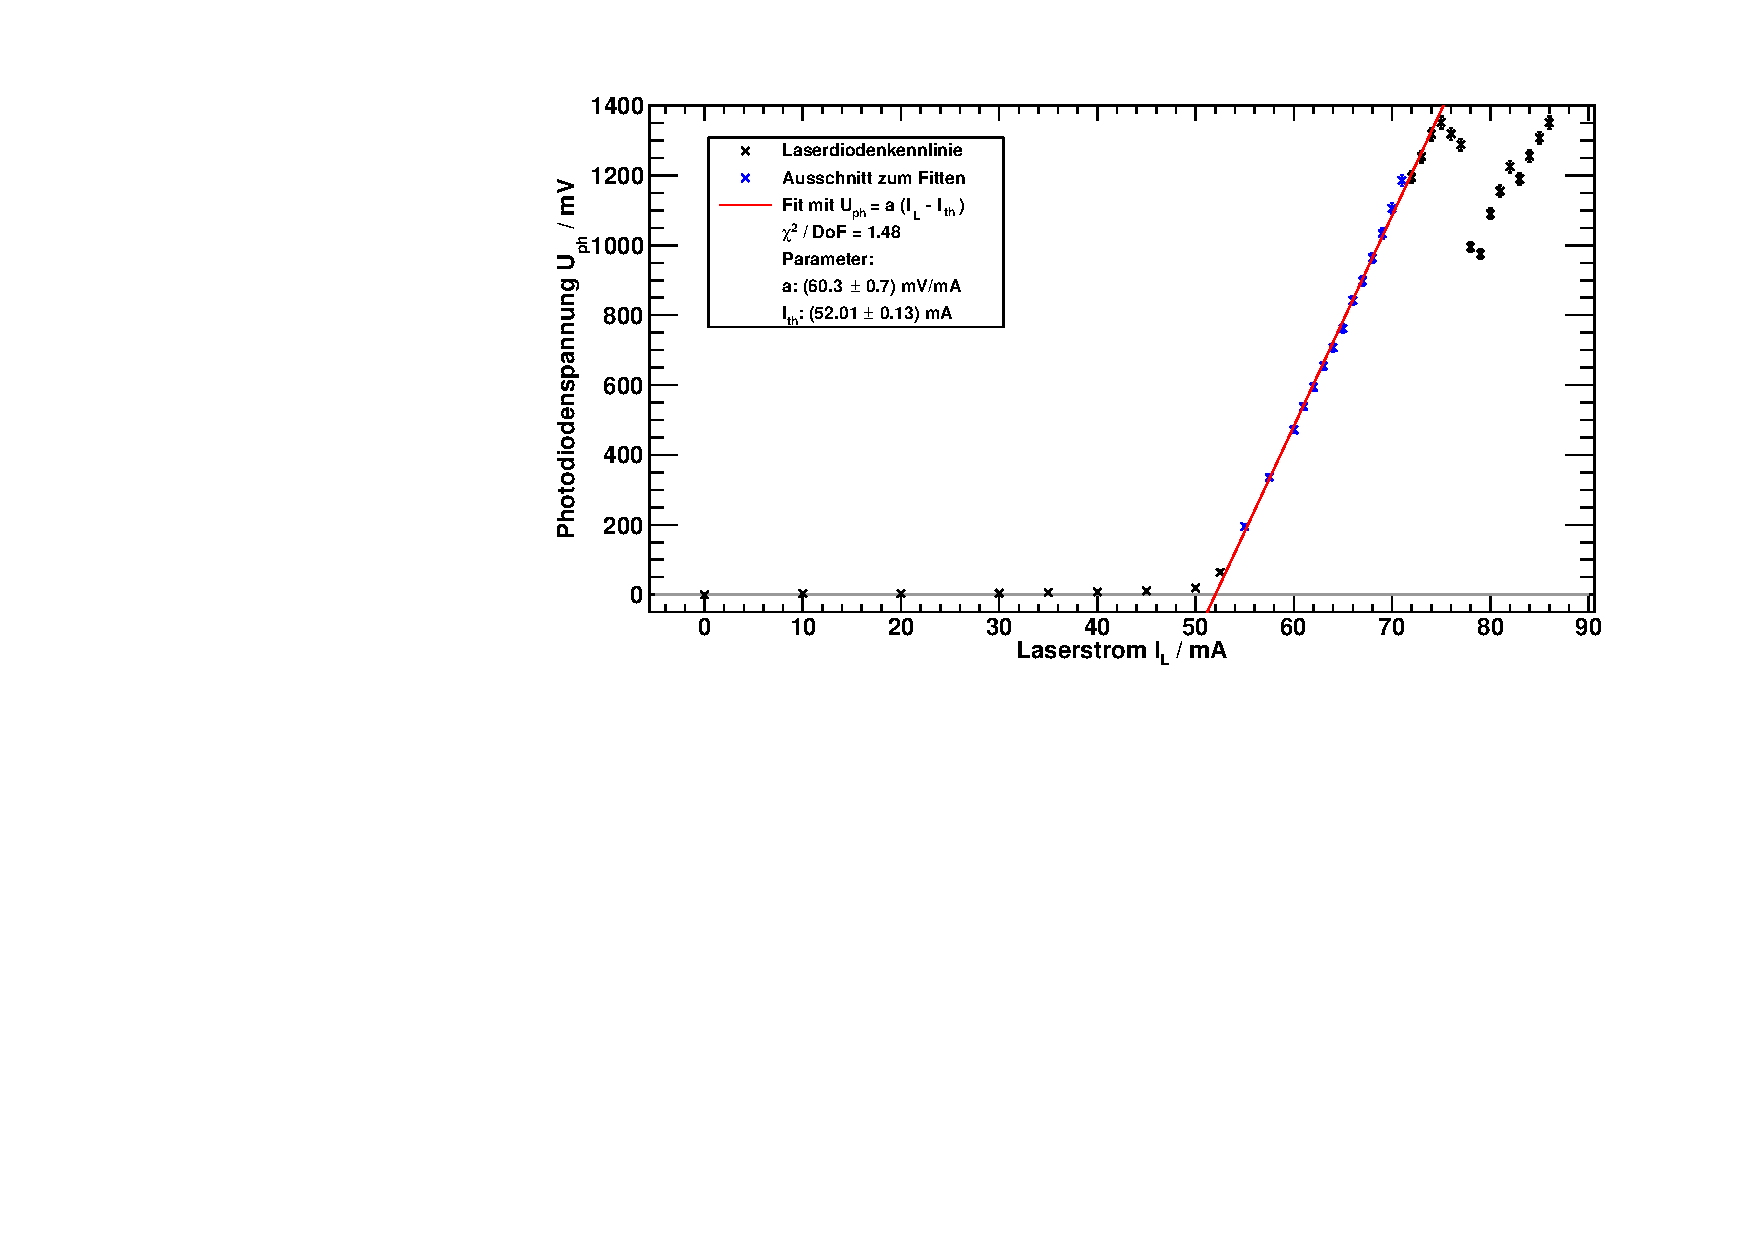
\includegraphics[width=\textwidth]{../img/diodenkennlinie.pdf}
        \caption{$P$-$I$-Kennlinie der im Versuch verwendeten Laserdiode.}
    \end{center}
\end{figure}
\end{frame}


\begin{frame}
\frametitle{Laserdiode - Aufbau zur Charakterisierung}
\setbeamerfont{myfont}{size*=80}
\usebeamerfont{myfont}
\begin{figure}
    \centering
    \def\svgwidth{\textwidth}
    \input{../img/aufbauEtalon.pdf_tex}
    \caption{Aufbau zur Identifikation von Modensprüngen der Laserdiode.}
\end{figure}
\usebeamerfont{standard}
\begin{itemize}
  \item \textbf{Etalon:} Transmissionsmaxima mit bekanntem Abstand
\end{itemize}
\end{frame}


\begin{frame}
\frametitle{Laserdiode - Frequenzmodulation}
\begin{figure}[H]
    \begin{center}
        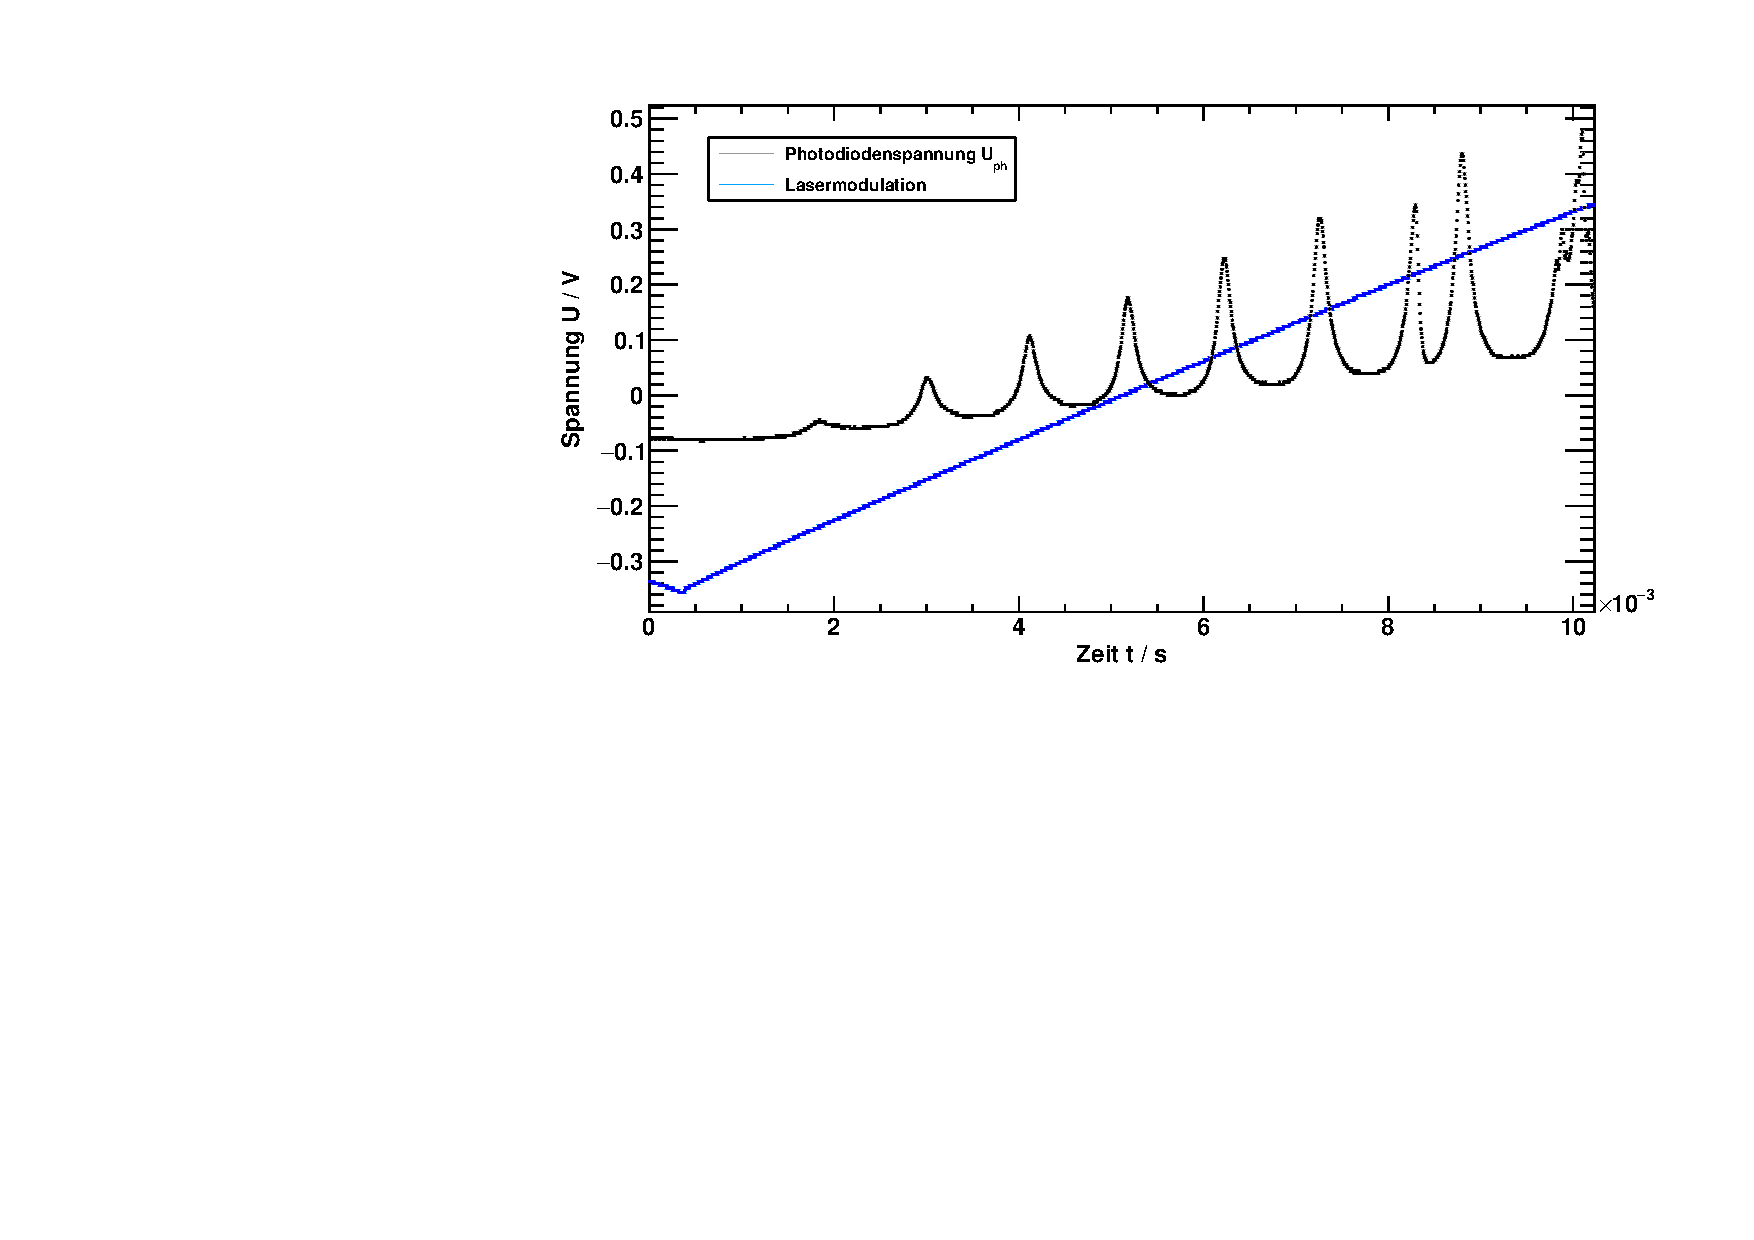
\includegraphics[width=\textwidth]{../img/up-etalon_zoom.pdf}
        \caption{Frequenzabhängige Transmission des Laserlichts durch das Etalon.}
    \end{center}
\end{figure}
\end{frame}


\begin{frame}
\frametitle{Laserdiode - Frequenzmodulation}

\begin{figure}[H]
    \begin{center}
        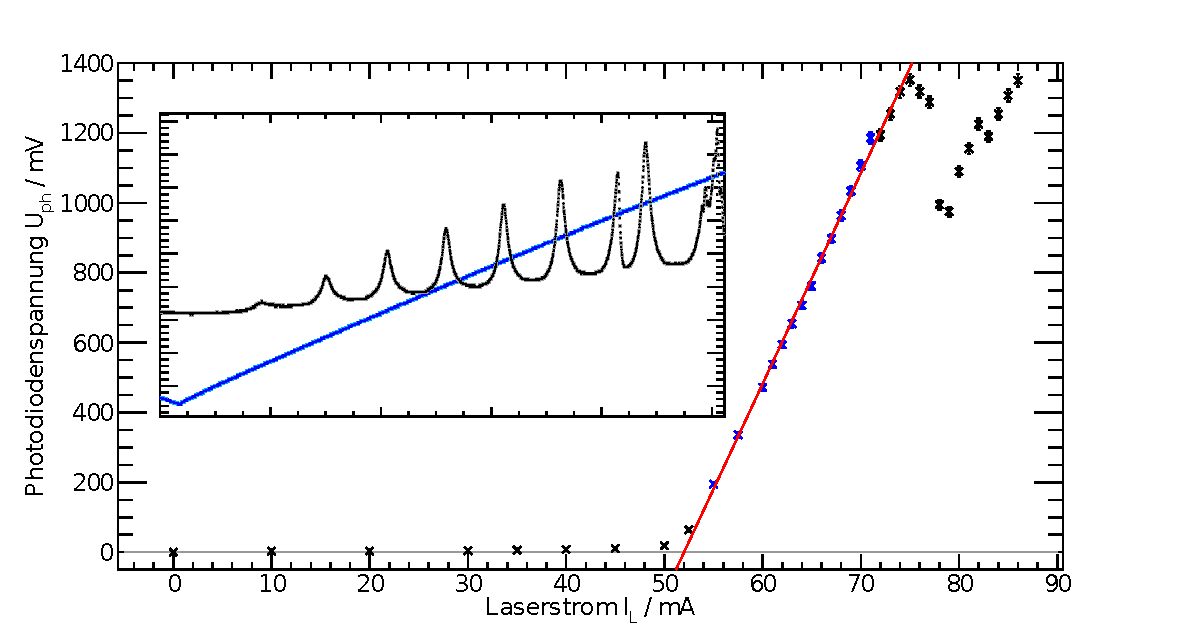
\includegraphics[width=\textwidth]{../img/diodenkennlinie+etalonspect.pdf}
        \caption{Vergleich von Frequenz und Leistung der Laserdiode.}
    \end{center}
\end{figure}
\end{frame}





\section{Introduction}

\subsection[Short First Subsection Name]{First Subsection Name}

\begin{frame}
\frametitle{}
\framesubtitle{Subtitles are optional}

\begin{itemize}
  \item
  \item
\end{itemize}
\end{frame}

\begin{frame}
\frametitle{}

% You can create overlays
\begin{itemize}
  \item using the \texttt{pause} command:
  \begin{itemize}
    \item First item.
    \pause
    \item Second item.
  \end{itemize}
  \item using overlay specifications:
  \begin{itemize}
    \item<3-> First item.
    \item<4-> Second item.
  \end{itemize}
  \item using the general \texttt{uncover} command:
  \begin{itemize}
    \uncover<5->{\item First item.}
    \uncover<6->{\item Second item.}
  \end{itemize}
\end{itemize}
\end{frame}

\section*{Summary}

\begin{frame}
\frametitle<presentation>{Summary}

\begin{itemize}
  \item The \alert{first main message} of your talk in one or two lines.
\end{itemize}

% The following outlook is optional.
\vskip0pt plus.5fill
\begin{itemize}
  \item Outlook
  \begin{itemize}
    \item Something you haven't solved.
    \item Something else you haven't solved.
  \end{itemize}
\end{itemize}
\end{frame}

\end{document}
